\chapter{Conservation of Mass and Balanced Equations}\label{ch:g8:balanced-equations}

A log weighing two kilograms burns in a fireplace. In the morning, a few
tens of grams of grey ash are left. Did almost two kilograms of matter
vanish in the night? For centuries nobody could say. The answer came
from a chemist who decided to weigh everything --- including the gases
that nobody had thought of weighing.

\begin{recall}
In a \omterm{def:g7:chemical-reactions:reaction}{chemical reaction} the \omterm{def:g7:chemical-reactions:reactant}{reactants} are used up and the products are
formed; the \omterm{def:g7:atoms-and-molecules:atom}{atoms} of the \omterm{def:g7:chemical-reactions:reactant}{reactants} are rearranged into the products,
neither created nor destroyed (\cref{ch:g7:chemical-reactions}). A
\omterm{def:g7:atoms-and-molecules:formula}{chemical formula} such as \ce{H2O} lists the \omterm{def:g7:atoms-and-molecules:atom}{atoms} of a \omterm{def:g7:atoms-and-molecules:molecule}{molecule}; a
number in front, as in \ce{3H2O}, counts \omterm{def:g7:atoms-and-molecules:molecule}{molecules}
(\cref{ch:g7:atoms-and-molecules}).
\end{recall}

\begin{omfigure}
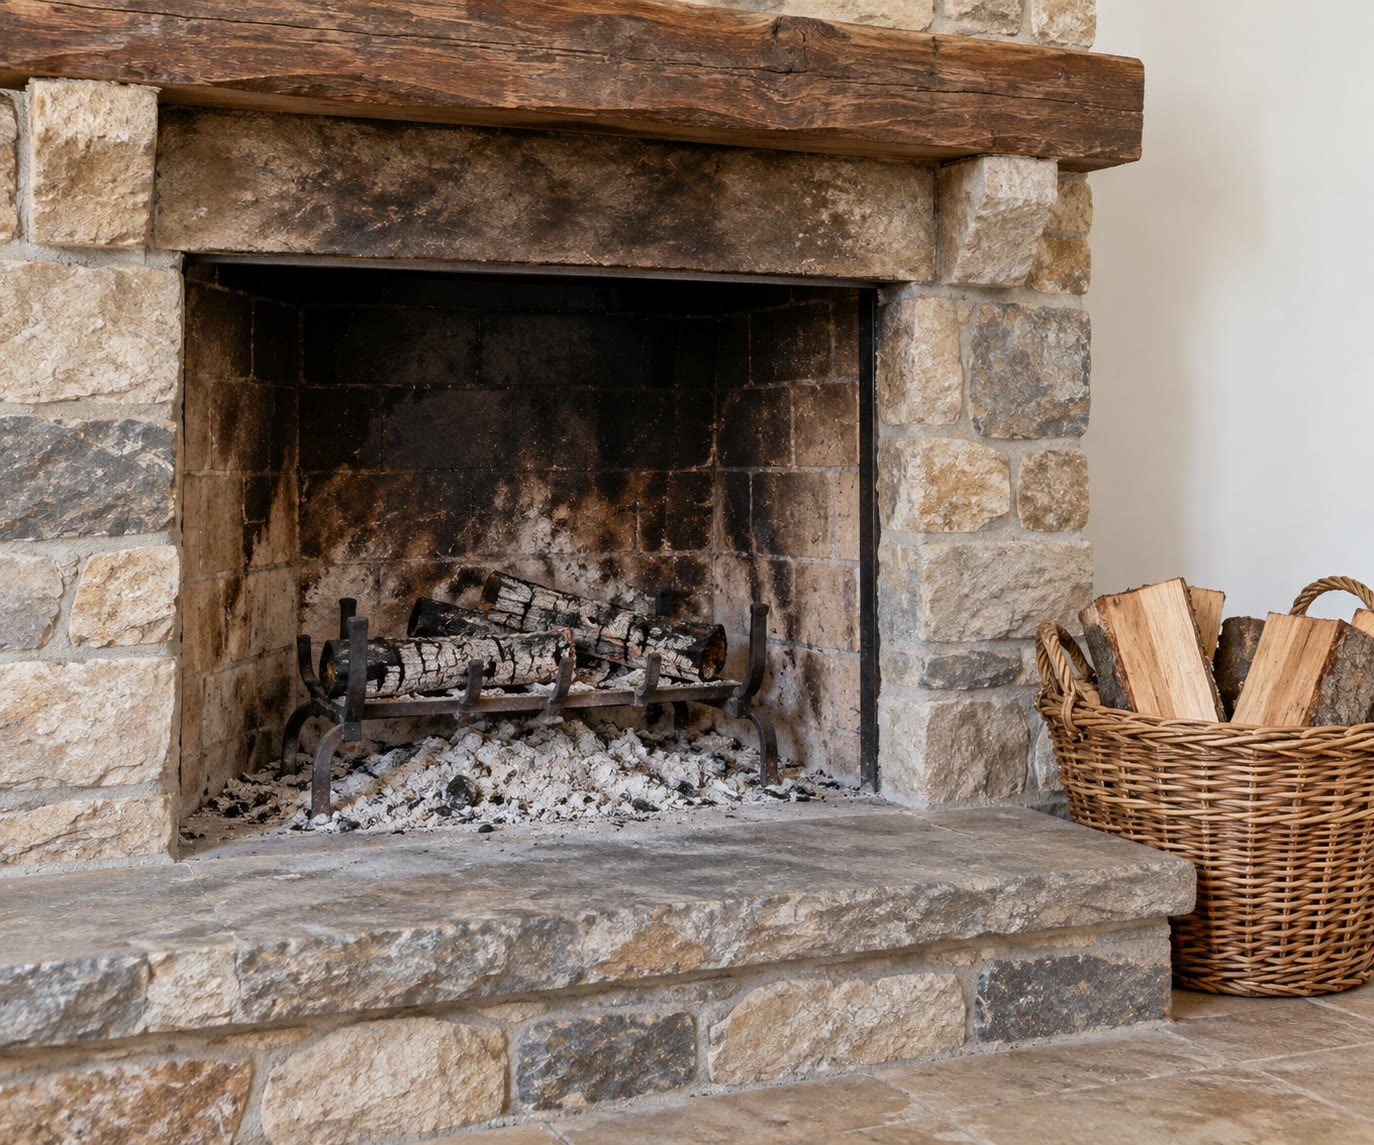
\includegraphics[width=0.5\linewidth]{images/book1/ai/g8-fireplace-ash.jpg}

{\small A fireplace the morning after: a little ash is all that is left
of the logs.}
\end{omfigure}

\section{Mass is conserved}

\begin{inthelab}[Weighing a reaction in a closed flask]
The teacher puts some vinegar in a flask, and baking soda in a balloon
fitted over its neck, then sets the whole on a balance: \qty{212.4}{g}.
The balloon is lifted so that the soda falls into the vinegar: the
\omterm{def:g6:pure-substances-and-mixtures:mixture}{mixture} fizzes and the balloon swells with the gas formed. The balance
still reads \qty{212.4}{g}. The same reaction in an open flask, without
the balloon, ``loses'' mass: the gas escapes into the room.
\end{inthelab}

\begin{omfigure}
\begin{tikzpicture}[font=\small, scale=1.15]
  % closed flask
  \pic[transform shape] at (0,0) {balance};
  \pic[transform shape] at (0,0.8) {erlenmeyer={0.25}{omWater!80}};
  \fill[red!55, draw=red!60!black] (0,4.05) ellipse (0.5 and 0.62);
  \fill[red!55] (-0.3,3.45) rectangle (0.3,3.6);
  \node[anchor=north, align=center] at (0,-0.1) {closed: the gas stays\\ in the balloon};
  \node[anchor=west, font=\footnotesize] at (1.25,0.3) {\qty{212.4}{g}};
  % open flask
  \pic[transform shape] at (4,0) {balance};
  \pic[transform shape] at (4,0.8) {erlenmeyer={0.25}{omWater!80}};
  \foreach \y in {3.6,3.95,4.3} \draw[->, black!45, decorate,
    decoration={snake, amplitude=0.6pt, segment length=4pt}] (4,\y) -- (4,\y+0.3);
  \node[anchor=north, align=center] at (4,-0.1) {open: the gas escapes,\\ the reading drops};
  \node[anchor=west, font=\footnotesize] at (5.25,0.3) {\qty{211.9}{g}};
\end{tikzpicture}

{\small The same reaction, weighed. In the closed flask the mass does
not change; in the open flask the gas leaves and the balance reads
less.}
\end{omfigure}

\begin{definition}[Conservation of mass]\label{def:g8:balanced-equations:conservation}
\emph{Conservation of mass}\index{conservation of mass} is the law that
in a \omterm{def:g7:chemical-reactions:reaction}{chemical reaction}, the total mass of the products formed is equal
to the total mass of the \omterm{def:g7:chemical-reactions:reactant}{reactants} used up. Nothing is lost and nothing
is created; matter only changes form.
\end{definition}

\begin{example}[The log, weighed properly]\label{ex:g8:balanced-equations:log}
If the \omterm{def:g4:what-a-fire-needs:burning}{burning} log and the oxygen it took from the \omterm{def:g4:air-a-mixture-of-gases:air}{air} could be weighed
before, and the ash, carbon dioxide and water vapour after, the two
totals would be equal. The ash is light because most of the products
are gases that go up the chimney.
\end{example}

\begin{history}[Lavoisier weighs everything, 1770s--1789]
Antoine-Laurent Lavoisier made a rule of weighing
every substance before and after each reaction, in sealed vessels so
that no gas could escape or enter. He showed that metals gain mass when
they rust or burn, by taking something from the \omterm{def:g4:air-a-mixture-of-gases:air}{air} --- oxygen, which
he named --- and stated in 1789 that nothing is created and nothing is
lost in a reaction. His wife, Marie-Anne Paulze Lavoisier, worked beside
him, recorded the experiments and drew the apparatus for his book.
\end{history}

\begin{omfigure}
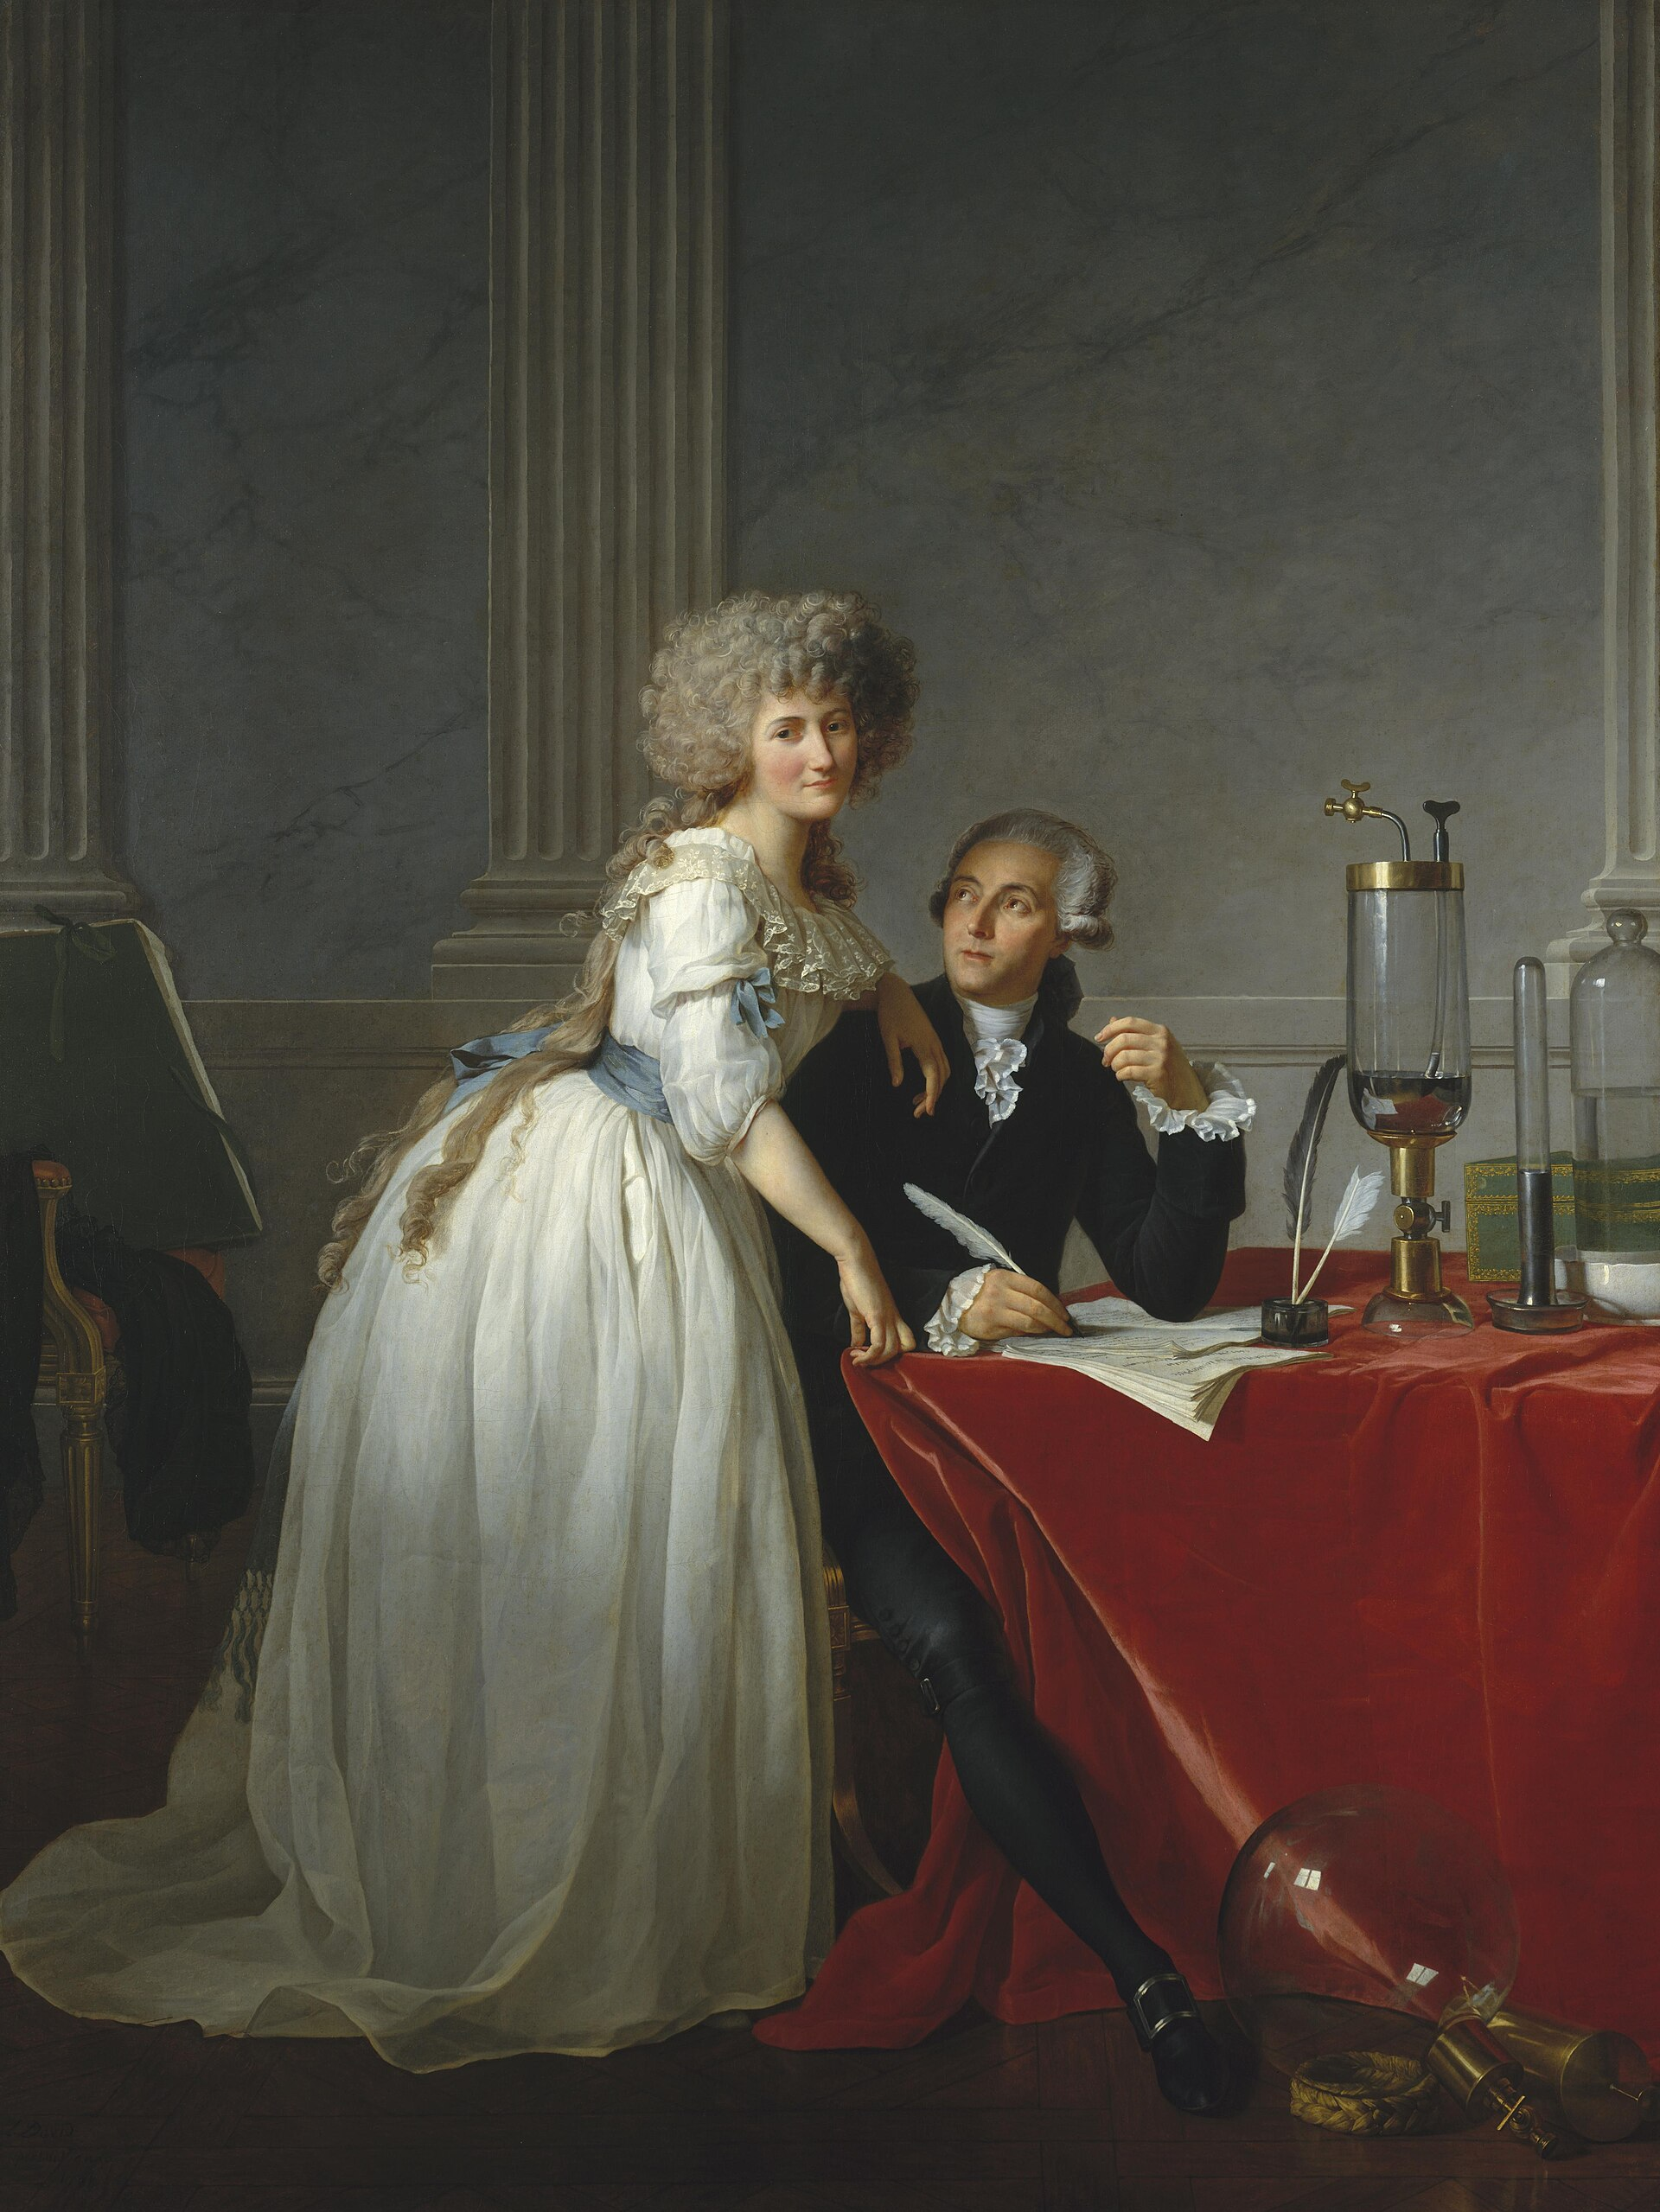
\includegraphics[width=0.3\linewidth]{images/book1/lavoisier.jpg}

{\small Antoine-Laurent Lavoisier and Marie-Anne Paulze Lavoisier, by
Jacques-Louis David, 1788.}
\end{omfigure}

\section{Why mass is conserved}

\begin{proposition}[Atoms are conserved, so mass is conserved]\label{prop:g8:balanced-equations:why}
In a reaction the \omterm{def:g7:atoms-and-molecules:atom}{atoms} are only rearranged: every \omterm{def:g7:atoms-and-molecules:atom}{atom} of the
\omterm{def:g7:chemical-reactions:reactant}{reactants} is found again in the products. Each \omterm{def:g7:atoms-and-molecules:atom}{atom} keeps its own mass.
The total mass therefore cannot change.
\end{proposition}

\begin{example}[Iron that gains mass]\label{ex:g8:balanced-equations:iron}
Steel wool burnt on a balance in an open dish gets heavier: the iron
\omterm{def:g7:atoms-and-molecules:atom}{atoms} have joined oxygen \omterm{def:g7:atoms-and-molecules:atom}{atoms} taken from the \omterm{def:g4:air-a-mixture-of-gases:air}{air}, and the iron oxide
formed weighs the iron plus that oxygen. Burnt in a sealed jar of \omterm{def:g4:air-a-mixture-of-gases:air}{air} on
the balance, the whole does not change mass: the oxygen was already
inside the jar.
\end{example}

\section{The chemical equation}

\begin{definition}[Chemical equation]\label{def:g8:balanced-equations:equation}
A \emph{chemical equation}\index{chemical equation} writes a reaction
with formulas: the formulas of the \omterm{def:g7:chemical-reactions:reactant}{reactants} on the left, joined by
$+$, an arrow, and the formulas of the products on the right. Each
formula may carry a number in front of it. The equation is a
\emph{balanced equation}\index{balanced equation} when each kind of \omterm{def:g7:atoms-and-molecules:atom}{atom}
appears the same number of times on both sides.
\end{definition}

\begin{definition}[Stoichiometric coefficient]\label{def:g8:balanced-equations:coefficient}
The number written in front of a formula in an equation is its
\emph{stoichiometric coefficient}\index{stoichiometric coefficient}: it
counts the \omterm{def:g7:atoms-and-molecules:molecule}{molecules} (or other particles) of that species taking part.
A coefficient 1 is not written.
\end{definition}

\begin{notation}[State symbols]\label{not:g8:balanced-equations:states}
A letter in brackets after a formula may give its physical state:
(s) solid, (l) liquid, (g) gas. Thus \ce{H2O(l)} is liquid water and
\ce{H2O(g)} water vapour.
\end{notation}

\begin{example}[Reading an equation]\label{ex:g8:balanced-equations:read}
\[
  \ce{CH4(g) + 2O2(g) -> CO2(g) + 2H2O(l)}
\]
reads: one methane \omterm{def:g7:atoms-and-molecules:molecule}{molecule} and two oxygen \omterm{def:g7:atoms-and-molecules:molecule}{molecules} react to give one
carbon dioxide \omterm{def:g7:atoms-and-molecules:molecule}{molecule} and two water \omterm{def:g7:atoms-and-molecules:molecule}{molecules}. Left: 1 C, 4 H, 4 O.
Right: 1 C, 4 H, $2 + 2 = 4$ O. The equation is balanced.
\end{example}

\begin{omfigure}
\begin{tikzpicture}[font=\small]
  \begin{scope}[every node/.style={font=\Large, inner sep=2pt}]
    \node (a) at (0,0) {\ce{CH4}};
    \node (p1) at (0.95,0) {$+$};
    \node (b) at (1.9,0) {\ce{2O2}};
    \node (arr) at (3.35,0) {$\longrightarrow$};
    \node (c) at (4.8,0) {\ce{CO2}};
    \node (p2) at (5.75,0) {$+$};
    \node (d) at (6.8,0) {\ce{2H2O}};
  \end{scope}
  \draw[thick, omDef] ([yshift=-2pt]a.south west) -- ++(0,-0.15) -| ([yshift=-2pt]b.south east);
  \node[below=8pt, text=black] at ($(a.south)!0.5!(b.south)$) {reactants};
  \draw[thick, omProp] ([yshift=-2pt]c.south west) -- ++(0,-0.15) -| ([yshift=-2pt]d.south east);
  \node[below=8pt, text=black] at ($(c.south)!0.5!(d.south)$) {products};
  \node[above=6pt of arr, font=\small] {``react to give''};
  \node[anchor=north west, align=left, draw=black!35, rounded corners=2pt,
    font=\small, inner sep=4pt] at (-0.3,-1.25)
    {In \ce{2O2}: the large 2 in front is the \textbf{coefficient} (two molecules);\\
     the small 2 below the line is the \textbf{subscript} (two atoms in each molecule).};
\end{tikzpicture}

{\small The parts of a \omterm{def:g8:balanced-equations:equation}{chemical equation}.}
\end{omfigure}

\section{Balancing an equation}

\begin{method}[Balancing an equation]\label{met:g8:balanced-equations:balance}
\begin{enumerate}
  \item Write the correct formulas of the \omterm{def:g7:chemical-reactions:reactant}{reactants} and products. Never
        change a formula afterwards: changing \ce{H2O} into \ce{H2O2}
        would describe another substance.
  \item Count the \omterm{def:g7:atoms-and-molecules:atom}{atoms} of each kind on each side.
  \item Balance one kind of \omterm{def:g7:atoms-and-molecules:atom}{atom} at a time with coefficients, starting
        with the \omterm{def:g7:atoms-and-molecules:atom}{atoms} that appear in only one formula on each side;
        leave hydrogen and oxygen for last.
  \item Count again; repeat until every kind of \omterm{def:g7:atoms-and-molecules:atom}{atom} balances.
  \item Use the smallest whole numbers.
\end{enumerate}
\end{method}

\begin{example}[Hydrogen and oxygen]\label{ex:g8:balanced-equations:water}
Unbalanced: \ce{H2 + O2 -> H2O} % ce-unbalanced-ok (the skeleton)
has 2 O on the left, 1 on the right. Put 2 in front of \ce{H2O}: now 4 H
on the right, so 2 in front of \ce{H2}:
\[
  \ce{2H2 + O2 -> 2H2O}.
\]
Check: 4 H and 2 O on each side.
\end{example}

\begin{example}[Iron burning in oxygen]\label{ex:g8:balanced-equations:iron-oxide}
Iron and oxygen give the iron oxide \ce{Fe2O3}. Oxygen: 2 on the left,
3 on the right; the smallest common number is 6, so 3 \ce{O2} and 2
\ce{Fe2O3}. Then 4 Fe on the right, so 4 Fe on the left:
\[
  \ce{4Fe + 3O2 -> 2Fe2O3}.
\]
\end{example}

\begin{omfigure}
\begin{tikzpicture}[font=\small]
  % 2 H2
  \foreach \y in {0.45,-0.45} {
    \node[aH] (a) at (0,\y) {}; \node[aH] (b) at (0.45,\y) {};
    \begin{scope}[on background layer]\draw[bond] (a.center) -- (b.center);\end{scope}}
  \node at (1.05,0) {$+$};
  \node[aO] (a) at (1.6,0) {}; \node[aO] (b) at (2.25,0) {};
  \begin{scope}[on background layer]
    \draw[bond, line width=1.1pt] ([yshift=1.6pt]a.center) -- ([yshift=1.6pt]b.center);
    \draw[bond, line width=1.1pt] ([yshift=-1.6pt]a.center) -- ([yshift=-1.6pt]b.center);
  \end{scope}
  \draw[->, thick, omProp] (2.9,0) -- (3.9,0);
  \foreach \y in {0.5,-0.5} {
    \node[aO] (o) at (4.9,\y+0.12) {};
    \node[aH] (p) at (4.35,\y-0.28) {}; \node[aH] (q) at (5.45,\y-0.28) {};
    \begin{scope}[on background layer]
      \draw[bond] (o.center) -- (p.center); \draw[bond] (o.center) -- (q.center);
    \end{scope}}
  \node[align=center, font=\footnotesize] at (1.1,-1.35) {4 H, 2 O};
  \node[align=center, font=\footnotesize] at (4.9,-1.35) {4 H, 2 O};
  \node[font=\small] at (2.7,-2.0) {\ce{2H2 + O2 -> 2H2O}};
\end{tikzpicture}

{\small The \omterm{def:g8:balanced-equations:equation}{balanced equation} of hydrogen \omterm{def:g4:what-a-fire-needs:burning}{burning}, drawn with models:
two hydrogen \omterm{def:g7:atoms-and-molecules:molecule}{molecules} and one oxygen \omterm{def:g7:atoms-and-molecules:molecule}{molecule} give two water
\omterm{def:g7:atoms-and-molecules:molecule}{molecules}.}
\end{omfigure}

\section{Reading an equation in molecules}


\begin{proposition}[What a balanced equation says]\label{prop:g8:balanced-equations:molecules}
The coefficients of a \omterm{def:g8:balanced-equations:equation}{balanced equation} give the proportions in which
the particles react and are formed. If the equation reads
\ce{2H2 + O2 -> 2H2O}, then 200 hydrogen \omterm{def:g7:atoms-and-molecules:molecule}{molecules} react with 100
oxygen \omterm{def:g7:atoms-and-molecules:molecule}{molecules} to give 200 water \omterm{def:g7:atoms-and-molecules:molecule}{molecules}; a million oxygen \omterm{def:g7:atoms-and-molecules:molecule}{molecules}
need two million hydrogen \omterm{def:g7:atoms-and-molecules:molecule}{molecules}.
\end{proposition}

\begin{example}[Propane in a camping stove]\label{ex:g8:balanced-equations:propane}
Propane, \ce{C3H8}, burns in oxygen to give carbon dioxide and water.
Carbon first: 3 C, so 3 \ce{CO2}. Hydrogen: 8 H, so 4 \ce{H2O}. Oxygen
on the right: $3 \times 2 + 4 = 10$ O, so 5 \ce{O2}:
\[
  \ce{C3H8 + 5O2 -> 3CO2 + 4H2O}.
\]
Each propane \omterm{def:g7:atoms-and-molecules:molecule}{molecule} needs five oxygen \omterm{def:g7:atoms-and-molecules:molecule}{molecules}.
\end{example}

\section{Exercises}

\begin{exercise}[$\star$]\label{exo:g8:balanced-equations:1}
State the law of \omterm{def:g8:balanced-equations:conservation}{conservation of mass}.
\end{exercise}

\begin{exercise}[$\star$]\label{exo:g8:balanced-equations:2}
In \ce{3CO2}, what is the \omterm{def:g8:balanced-equations:coefficient}{stoichiometric coefficient}? How many carbon
\omterm{def:g7:atoms-and-molecules:atom}{atoms} and how many oxygen \omterm{def:g7:atoms-and-molecules:atom}{atoms} does it represent?
\end{exercise}

\begin{exercise}[$\star$]\label{exo:g8:balanced-equations:3}
Is \ce{C + O2 -> CO2} balanced? Count the \omterm{def:g7:atoms-and-molecules:atom}{atoms} to check.
\end{exercise}

\begin{exercise}[$\star$]\label{exo:g8:balanced-equations:4}
Balance \ce{Mg + O2 -> MgO}. % ce-unbalanced-ok (to balance)
\end{exercise}

\begin{exercise}[$\star\star$]\label{exo:g8:balanced-equations:5}
Balance \ce{N2 + H2 -> NH3}, the reaction that makes ammonia. % ce-unbalanced-ok (to balance)
\end{exercise}

\begin{exercise}[$\star\star$]\label{exo:g8:balanced-equations:6}
\qty{12}{g} of carbon burn completely and form \qty{44}{g} of carbon
dioxide. What mass of oxygen was used?
\end{exercise}

\begin{exercise}[$\star\star$]\label{exo:g8:balanced-equations:7}
Look at the figure of the two flasks on balances. Why does the reading
of the open flask drop? Has mass been destroyed?
\end{exercise}

\begin{exercise}[$\star\star$]\label{exo:g8:balanced-equations:8}
Balance \ce{CH4 + O2 -> CO2 + H2O} step by step, saying which \omterm{def:g7:atoms-and-molecules:atom}{atom} you % ce-unbalanced-ok (to balance)
balance at each step.
\end{exercise}

\begin{exercise}[$\star\star$]\label{exo:g8:balanced-equations:9}
A student balances \ce{H2 + O2 -> H2O} by writing \ce{H2 + O2 -> H2O2}. % ce-unbalanced-ok (the student's start)
Why is this wrong?
\end{exercise}

\begin{exercise}[$\star\star$]\label{exo:g8:balanced-equations:10}
Using \ce{C3H8 + 5O2 -> 3CO2 + 4H2O}, how many oxygen \omterm{def:g7:atoms-and-molecules:molecule}{molecules} are
needed to burn 20 propane \omterm{def:g7:atoms-and-molecules:molecule}{molecules}? How many water \omterm{def:g7:atoms-and-molecules:molecule}{molecules} are
formed?
\end{exercise}

\begin{exercise}[$\star\star\star$]\label{exo:g8:balanced-equations:11}
Balance \ce{C2H6 + O2 -> CO2 + H2O}, the \omterm{def:g4:what-a-fire-needs:burning}{burning} of ethane. (Hint: try % ce-unbalanced-ok (to balance)
doubling the ethane.)
\end{exercise}

\begin{exercise}[$\star\star\star$]\label{exo:g8:balanced-equations:12}
A candle of \qty{20.0}{g} burns in a sealed glass box full of \omterm{def:g4:air-a-mixture-of-gases:air}{air}, which
sits on a balance reading \qty{850.0}{g} in all. When the flame goes out,
the candle weighs \qty{19.6}{g}. What does the balance read? Explain.
\end{exercise}

\section{Problem: Steel Wool in a Sealed Jar}

\begin{problem}[{Weekend problem --- iron that burns, a balance that does
not move, and the oxygen taken from the air}]
\label{pb:g8:balanced-equations:1}
In a laboratory, a teacher burns steel wool, which is almost pure iron,
in two ways. First, a pad is burnt in an open dish on a balance: the
reading goes up. Then a pad of \qty{0.28}{g} is burnt, ignited by an
electric spark, inside a closed jar of \omterm{def:g4:air-a-mixture-of-gases:air}{air} standing on the balance: the
reading does not change. The jar holds about \qty{0.5}{g} of oxygen.
Iron \omterm{def:g4:what-a-fire-needs:burning}{burning} in oxygen forms the iron oxide \ce{Fe2O3}; with less oxygen
it can also form \ce{Fe3O4}.

\medskip
\noindent\textbf{Part I --- Two weighings.}
\begin{enumerate}
  \item In the open dish, the mass goes up. Where does the extra mass
        come from?
  \item In the closed jar, the mass does not change. Explain.
  \item State the law illustrated by these two weighings.
\end{enumerate}

\medskip
\noindent\textbf{Part II --- Two equations.}
\begin{enumerate}[resume]
  \item Balance the equation \ce{Fe + O2 -> Fe2O3}. % ce-unbalanced-ok (to balance)
  \item Balance the equation \ce{Fe + O2 -> Fe3O4}. % ce-unbalanced-ok (to balance)
  \item Check the first equation by counting the \omterm{def:g7:atoms-and-molecules:atom}{atoms} of each kind on
        each side.
  \item According to the first equation, how many oxygen \omterm{def:g7:atoms-and-molecules:molecule}{molecules} react
        with 400 iron \omterm{def:g7:atoms-and-molecules:atom}{atoms}?
\end{enumerate}

\medskip
\noindent\textbf{Part III --- Masses.}
In \ce{Fe2O3}, every \qty{7}{g} of iron are combined with \qty{3}{g} of
oxygen. The \qty{0.28}{g} pad burns completely to \ce{Fe2O3}.
\begin{enumerate}[resume]
  \item What mass of oxygen combines with \qty{0.28}{g} of iron?
  \item What is the mass of iron oxide formed?
  \item Was there enough oxygen in the jar? Explain.
  \item The jar is opened after cooling, and \omterm{def:g4:air-a-mixture-of-gases:air}{air} rushes in. Explain why,
        and say how the reading of the balance then changes.
  \item Compute the mass of oxygen taken from the \omterm{def:g4:air-a-mixture-of-gases:air}{air} of the jar by the
        \omterm{def:g4:what-a-fire-needs:burning}{burning} steel wool.
\end{enumerate}
\end{problem}
